
%%%%%%%%%%%%%%%%%%%%%%%%%%%%%%%%%%%%%%%%%%%%%%%%%%%%%%%%%%%%%%%%%%%%%%%%%%%%%%
% Copyright (c) 2003-2015 by University of Queensland
% http://www.uq.edu.au
%
% Primary Business: Queensland, Australia
% Licensed under the Open Software License version 3.0
% http://www.opensource.org/licenses/osl-3.0.php
%
% Development until 2012 by Earth Systems Science Computational Center (ESSCC)
% Development 2012-2013 by School of Earth Sciences
% Development from 2014 by Centre for Geoscience Computing (GeoComp)
%
%%%%%%%%%%%%%%%%%%%%%%%%%%%%%%%%%%%%%%%%%%%%%%%%%%%%%%%%%%%%%%%%%%%%%%%%%%%%%%

\section{Darcy Flux}
\label{DARCY FLUX}
We want to calculate the flux $u$ and pressure $p$ on a domain $\Omega$
solving the Darcy flux problem\index{Darcy flux}\index{Darcy flow}
\begin{equation}\label{DARCY PROBLEM}
\begin{array}{rcl}
u_{i} + \kappa_{ij} p_{,j} & = & g_{i} \\
u_{k,k} & = & f
\end{array}
\end{equation} 
with the boundary conditions
\begin{equation}\label{DARCY BOUNDARY}
\begin{array}{rcl}
u_{i} \; n_{i}  = u^{N}_{i}  \; n_{i} & \mbox{ on } & \Gamma_{N} \\
p = p^{D} &  \mbox{ on } & \Gamma_{D} \\ 
\end{array}
\end{equation} 
where $\Gamma_{N}$ and $\Gamma_{D}$ are a partition of the boundary of
$\Omega$ with $\Gamma_{D}$ non-empty, $n_{i}$ is the outer normal field of the
boundary of $\Omega$, $u^{N}_{i}$ and $p^{D}$ are given functions on $\Omega$,
$g_{i}$ and $f$ are given source terms and $\kappa_{ij}$ is the given
permeability.
We assume that $\kappa_{ij}$ is symmetric (which is not really required) and
positive definite, i.e. there are positive constants $\alpha_{0}$ and
$\alpha_{1}$ which are independent from the location in $\Omega$ such that
\begin{equation}
\alpha_{0} \; x_{i} x_{i} \le \kappa_{ij} x_{i} x_{j} \le \alpha_{1} \; x_{i} x_{i}
\end{equation}
for all $x_{i}$.


\subsection{Solution Method \label{DARCY SOLVE}}
Unfortunate equation~\ref{DARCY PROBLEM} can not solved directly in an easy way and requires mixed FEM.  
We consider a few options to solve equation~\ref{DARCY PROBLEM}
\subsubsection{Evaluation}\label{SEC DARCY SIMPLE}
The first equation of equation~\ref{DARCY PROBLEM} is inserted into the second one:
\begin{equation}\label{DARCY PROBLEM SIMPLE}
- (\kappa_{ij} p_{,j})_{,i}  =  f  - (g_{i})_{,i}
\end{equation} 

with boundary conditions
\begin{equation}\label{DARCY BOUNDARY SIMPLE}
\begin{array}{rcl}
\kappa_{ij} p_{,j} \; n_{i}  = ( g_{i} - u^{N}_{i} )  \; n_{i} & \mbox{ on } & \Gamma_{N} \\
p = p^{D} &  \mbox{ on } & \Gamma_{D} \\ 
\end{array}
\end{equation} 
Then the flux field is recovered by directly setting
\begin{equation}\label{DARCY PROBLEM SIMPLE FLUX}
 u_{j} = g_j -  \kappa_{ij} p_{,j}  
\end{equation} 
This simple recovery process will not ensure that the (numerically) calculated flux
meets the boundary conditions for flux or the incompressibility condition. 
However this is a very fast way of calculating the flux.


\subsubsection{Global Postprocessing \label{SEC DARCY POST}}
An improved flux recovery can be achieved by solving a modified version of equation~\ref{DARCY PROBLEM SIMPLE FLUX}
adding the gradient of the divergence of the flux:
\begin{equation}\label{DARCY PROBLEM POST FLUX}
\kappa^{-1}_{ij} u_{j} - 
(\lambda \cdot u_{k,k} )_{,i}= 
\kappa^{-1}_{ij} g_j- p_{,i} 
- (\lambda \cdot f )_{,i} 
\end{equation} 
where
\begin{equation}\label{DARCY PROBLEM POST FLUX A}
\lambda = \omega \cdot |\kappa^{-1}| \cdot vol(\Omega)^{1/d} \cdot h 
\end{equation} 
with a non-negative factor $\omega$, $d$ is the spatial dimension and $h$ is the local element size.
\begin{equation}\label{DARCY PROBLEM POST FLUX BOUNDARY}
\begin{array}{rcl}
u_{i} \; n_{i}  = u^{N}_{i}  \; n_{i} & \mbox{ on } & \Gamma_{N} \\
u_{k,k} = f & \mbox{ on } & \Gamma_{D} \\ 
\end{array}
\end{equation}   
Notice that the second condition is a natural boundary condition.
Global post-processing is more expense than direct pressure evaluation
however the flux is more accurate and asymptotic incompressibility
for mesh size towards zero can be shown, if $\omega>0$.


\subsection{Functions}
\begin{classdesc}{DarcyFlow}{domain, \optional{w=1., \optional{solver=\member{DarcyFlow.POST},  \optional{
useReduced=\True, \optional{ verbose=\True} } }}}
opens the Darcy flux problem\index{Darcy flux} on the \Domain domain. 
Reduced approximations for pressure and flux are used if \var{useReduced} is set.
Argument \var{solver} defines the solver method. 
If \var{verbose} is set some information are printed.
\var{w} defines the weighting factor $\omega$ for global post-processing of the flux (see equation~\ref{DARCY PROBLEM POST FLUX A}.)
\end{classdesc}

\begin{memberdesc}[DarcyFlow]{EVAL}
flux is calculated directly from pressure evaluation, see section~\ref{SEC DARCY SIMPLE}.
\end{memberdesc}

\begin{memberdesc}[DarcyFlow]{SMOOTH}
solver using global post-processing of flux with weighting factor $\omega=0$, see section~\ref{SEC DARCY POST}. 
\end{memberdesc}

\begin{memberdesc}[DarcyFlow]{POST}
solver using global post-processing of flux, see section~\ref{SEC DARCY POST}. 
\end{memberdesc}

\begin{methoddesc}[DarcyFlow]{setValue}{\optional{f=None, \optional{g=None, \optional{location_of_fixed_pressure=None, \optional{location_of_fixed_flux=None, 
\\\optional{permeability=None}}}}}}
assigns values to the model parameters. Values can be assigned using various
calls -- in particular in a time dependent problem only values that change
over time need to be reset. The permeability can be defined as a scalar
(isotropic), or a symmetric matrix (anisotropic).
\var{f} and \var{g} are the corresponding parameters in~\ref{DARCY PROBLEM}.
The locations and components where the flux is prescribed are set by positive
values in \var{location_of_fixed_flux}.
The locations where the pressure is prescribed are set by by positive values
of \var{location_of_fixed_pressure}.
The values of the pressure and flux are defined by the initial guess.
Notice that at any point on the boundary of the domain the pressure or the
normal component of the flux must be defined. There must be at least one point
where the pressure is prescribed.
The method will try to cast the given values to appropriate \Data class objects.
\end{methoddesc}

\begin{methoddesc}[DarcyFlow]{getSolverOptionsFlux}{}
returns the solver options used to solve the flux problems.
Use this \SolverOptions object to control the solution algorithms.
This option is only relevant if global postprocesing is used.
\end{methoddesc}

\begin{methoddesc}[DarcyFlow]{getSolverOptionsPressure}{}
returns a \SolverOptions object with the options used to solve the pressure
problems.
Use this object to control the solution algorithms.
\end{methoddesc}

\begin{methoddesc}[DarcyFlow]{solve}{u0,p0}
solves the problem and returns approximations for the flux $v$ and the pressure $p$.
\var{u0} and \var{p0} define initial guesses for flux and pressure.
Values marked by positive values \var{location_of_fixed_flux} and
\var{location_of_fixed_pressure}, respectively, are kept unchanged.
\end{methoddesc}

\begin{methoddesc}[DarcyFlow]{getFlux}{p, \optional{ u0 = None}}
returns the flux for a given pressure \var{p} where the flux is equal to \var{u0}
on locations where \var{location_of_fixed_flux} is positive,  see \member{setValue}.
Notice that \var{g} and \var{f} are used.
\end{methoddesc}

\begin{figure}
\centerline{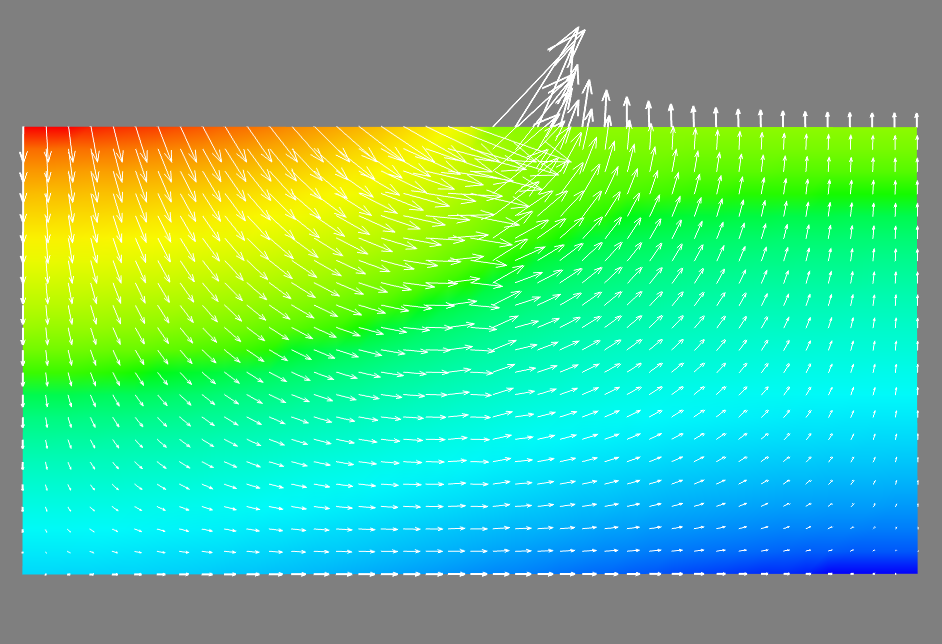
\includegraphics[width=\figwidth]{darcy_result}}
\caption{Flux and pressure field of the Dary flow example.}
\label{DARCY FIG 1}
\end{figure}

\subsection{Example: Gravity Flow}
The following script \file{darcy.py}\index{scripts!\file{darcy.py.py}}\index{Darcy flow}
which is available in the \ExampleDirectory illustrates the usage of the
\class{DarcyFlow} class:
\begin{python}
   from esys.escript import *
   from esys.escript.models import DarcyFlow
   from esys.finley import Rectangle
   from esys.weipa import saveVTK
   mydomain = Rectangle(l0=2.,l1=1.,n0=40, n1=20)
   x = mydomain.getX()
   p_BC=whereZero(x[1]-1.)*wherePositive(x[0]-1.)
   u_BC=(whereZero(x[0])+whereZero(x[0]-2.)) * [1.,0.] + \
     (whereZero(x[1]) + whereZero(x[1]-1.)*whereNonPositive(x[0]-1.0)) * [0., 1.]
   mypde = DarcyFlow(domain=mydomain)
   mypde.setValue(g=[0., 2],
                  location_of_fixed_pressure=p_BC,
                  location_of_fixed_flux=u_BC,
                  permeability=100.)

   u,p=mypde.solve(u0=x[1]*[0., -1.], p0=0)
   saveVTK("u.vtu",flux=u, pressure=p)
\end{python}
In the example the pressure is fixed to the initial pressure \var{p0} on the right half of the top face.
The normal flux is set on all other faces. The corresponding values for the flux are set by the initial value
\var{u0}.   
